\chapter{Hardware}
% ------------------------

%XXX: ALL THE FIGURES THAT HAVE NOT BEEN DRAWN BY YOURSELF NEED TO BE PROPERLY ACKNOWLEDGED AND REFERENCED!!!!!!!

\section{PCB (interface board)}
For the chip tester, two PCBs are needed in this project. One which is called B2
has been designed for the virtual designs to be loaded in a slave FPGA.

The other is called B1 and interfaces with the final fabricated chip.

Both PCBs are two layer boards and designed using Allegro 16.3 PCB designer tools.
The dimensions of B1 and B2 are $98.93 mm* 68.5 mm$ and $81.28 mm * 68.33 mm$ and the minimum wire size is $8mils$.

\newpage
\subsection{B1 (DUT testing board)}

\subsubsection{DUT}

The superchip under test has the following specific features:
\begin{itemize}
 \item $16$ separate design sites
 \item $24$ digital input pins [$A0\dots A23$], shared between all design sites;
 \item $24$ digital output pins [$Q0\dots Q23$], shared between all design sites;
 \item $16$ separate VDD pins, one dedicated to each design site;
 \item $1$ global GND pin for all design sites and infrastructure circuitry;
 \item $1$ global VDD pin to power the site buffers and I/O pad ring;
 \item $68$-pin JLCC package (with 2 unused pins).
\end{itemize}

The chip is interfaced with the PCB by a 68WAY PLCC/JLCC socket. Power is
supplied by the $3.3V$ VDD from the DE2 board. The GND is also connected to the DE2 GND.

The shared I/Os are connected to the powered design site, and disconnected from the other
design sites. Hence a controllable power switch is included with a $4-16$ decoder and an
integrated power switch array.

The Q1 is the output of a ring oscillator. The frequency can be measured using the digital
frequency counter module on the main FPGA. However, to examine the analog properties of this output,
an analog part including a buffer, $3^{rd}$ order Butterworth filter and ADC with their own power supply is also included.


\subsubsection{Digital Part}

\paragraph{Decoder}

Although there are 16 design sites to be selected, by using a decoder the 16
signals can be generated from only 4 board-to-board signals, saving on routing, since only one
site is selected at a time.

The decoder used is $74HC4514$, a $4-to-16$ line decoder with latch. The input and output are active high.

\paragraph{Switch Array}

The switch array consists of four $TPS2095$ quad power-distribution switches.
One could simply use a CMOS transistor to realize a switch. However, with thermal sense,
current limit and charge pump, the $TPS2095$ switches are more reliable, stable, smooth
(minimum switching current surges) and relatively compact in scale.
The operation of a switch is simple: when EN pin is asserted, the OUT pin offers
the power with the same voltage in the IN pin. Otherwise the OUT pin is disconnected
from the input power. In one $TPS2095$ chip there are 4 such switches, the EN pins of which are all active high, matching the output of the decoder.


\subsubsection{Analog Part}

\begin{figure}
 \centering
 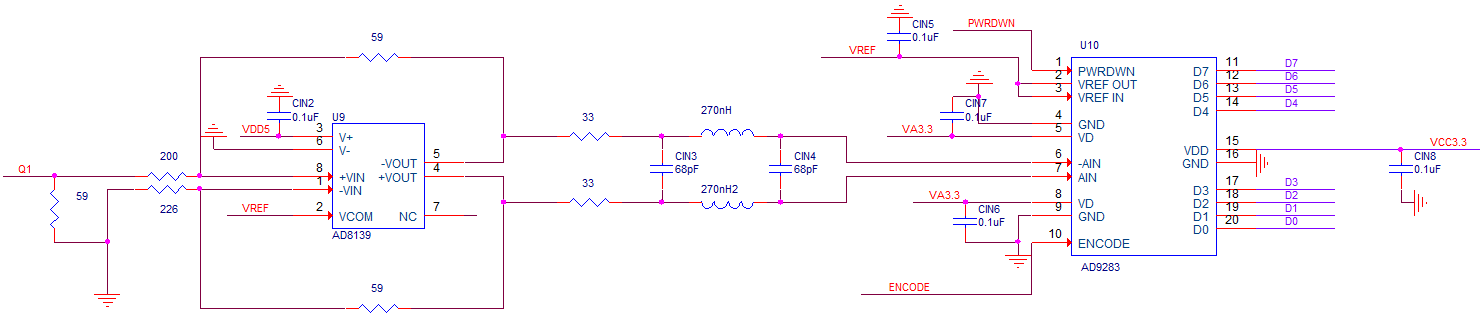
\includegraphics[width=0.95\textwidth]{analog_1}
 \caption{Analog Part Overview.}
 \label{fig:analog_overview}
\end{figure}

\paragraph{Buffer}
An $AD8139$ differential ADC driver is used as the front buffer of the ADC.
It is an ultralow noise, high performance differential amplifier with rail to rail
output from Analog Devices. The designed gain of the buffer is $0.295$, and the differential gain is approximately $0.14$. This allows
for single-ended input signals between 0 and 3.5V to be fed into the ADC which has a maximum differential range of $\pm 512 mV$.

\paragraph{ADC}
The $8-bit$, $100MSPS$ ADC is used to sample the analog signal. The encode clock is
the clock from the DE2 board ($100MHz$ by default).

A power-down function select is also connected to the FPGA for shutting down the ADC when it is not in use.
The ADC signal wires should be placed far away from the other wires for minimum interference;
and they should also be placed parallel to each other to have similar length for better signal integrity.
However, since the pin density of the HSMC connector used is high, it is inevitable that the ADC wires
are close to the other signal lines. The ADC is placed on the other side of the PCB board for a better result.


\paragraph{Butterworth Filter}
To minimize the high frequency noise and avoid aliasing from high frequency signals, a passive third-order low pass Butterworth filter
is used.

With three poles, the attenuation is $-60 \sfrac{dB}{decade}$ on signals higher than the cut-off frequency.
The filter topology used here is balanced ladder topology.
The automatic design tool Elsie was used for designing the parameters of the RCI circuit. The cut-off frequency is $40MHz$.
%XXX: bode plot of the filter!!!



\paragraph{Separate Power Supplies}
The buffer and ADC are separately powered from the other parts of the board to improve signal integrity.
The $AD8139$’s power ranges from $5V$ to $12V$, and the ADC ranges from $2.7V$ to $3.6V$.
Two low dropout regulators (LDP), $ADP3335$ and $ADP3333$ are used to offer $5V$ and $3.3V$ voltages respectively from the $12V$ power rail
on the HSMC connector.

The supply voltage of these two LDP ranges from $2.6V$ to $12V$. Their load currents are up to $500mA$ and $300mA$ respectively.


\newpage
\subsection{B2 (Virtual design board)}

When we started designing the B2 board for slave FPGA, the Altera PowerPlay Early Power Estimator was
used for early power estimation calculations.

An almost full usage of the slave FPGA, $90\%$ of all of logic blocks/cells,
$90\%$ of multipliers and $90\%$ of memory elements, as well as $64$ I/O pins was assumed.

The clock rate was assumed to be $100MHz$. In case of the toggle rates, two figures are assumed here.
One set is $12.5\%$ on every net as a maximum toggle rate for the device while the
other is $30\%$ which is a large and unlikely to be realistic in the worst-case power consumption situation.

Ambient temperature was taken as $25^{\circ} C$ and no heat sink was assumed in the calculations, and no air flow (still air).

The power consumption result for $12.5\%$ toggle rate:
\begin{itemize}
 \item Logic: $0.235 W$
 \item RAM: $0.009 W$
 \item DSP: $0.032W$
 \item I/O: $0.023 W$
 \item PLL: $0.016 W$
 \item Clock: $0.135W$
 \item P\_static: $0.123W$
 \item Total: $\approx0.574 W$
\end{itemize}
For $30\%$ toggle rate the main change is the change in Logic power consumption, therefore the consumption of Logic is $0.565 W$ and the Total is now $0.905 W$.

Translating these into power supply current requirements, for $12.5\%$ toggle rate:
\begin{itemize}
 \item Icc (int) ($1.2V$) $0.352A$
 \item Icc (A) ($2.5V$) $0.036A$
 \item Icc (d) ($1.2V$) $0.014A$
 \item Icc (IO) ($3.3V$) $0.013A$
\end{itemize}

For $30\%$ toggle rate the main change is Icc (int), changes to $0.627A$.

The current consumption the main board provides is $1.5A$ in $3.3V$ power supply
with a $50\%$ usage of the FPGA, which is sufficient for both cases since only $20\%$
is occupied in this project.


\subsubsection{Slave FPGA}
The slave FPGA is the core chip of the virtual design board. It can be configured
with HDL descriptions of the circuits to be tested.
An Altera Cyclone III FPGA will be chosen as the slave FPGA.

The reason for choosing Cyclone III is their low power, high functionality and low cost. By choosing
an Altera FPGA, the design flow will be similar to other FPGA systems used within the department.

A 144-pin EQFP package was chosen as it is easier to assemble than BGA packages and offers enough I/O
for use with the chip tester. I/O pins on the Cyclone III are grouped together into I/O banks,
and each bank has a separate power bus.

There are eight I/O banks, as shown in figure \ref{fig:b2_f1} \citep{Altera:2011:cyclone3handbook}.
All single-ended I/O standards are supported in all banks except HSTL-12 Class II which is only supported in column banks.
The same case can be found in all differential I/O standards.

\begin{figure}
 \centering
 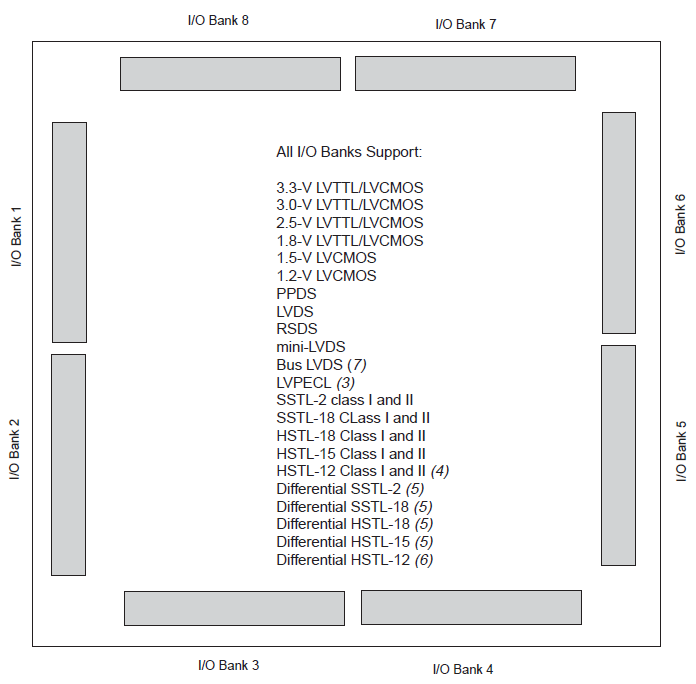
\includegraphics[width=0.9\textwidth]{figure1}
 \caption{I/O banks in Cyclone III FPGA. (from \citep{Altera:2011:cyclone3handbook})}
 \label{fig:b2_f1}
\end{figure}

In this design three voltage levels, which $VCCIO=3.3V$, $VCCINT= 1.2V$ and $VCCA=2.5V$, are necessary. These are provided
by low dropout linear regulators. Linear regulators offer better noise performance and require fewer external components.

Proper bypassing and decoupling techniques for the power pins is very important for reliable design operation.
In this case, additional decoupling capacitors were used on as many power pins as was possible to fit on the board.

In regard of the Cyclone III configuration, the device uses SRAM cells to
store configuration data. Since SRAM is volatile, an external configuration memory is required.
In AS mode, Cyclone III reads the configuration data from an external SPI flash. The SPI
flash is described in a later subsection.

The clock source for initialization is either a $10MHz$ (typical) internal oscillator or
an optional external oscillator on a CLK pin. In this situation, an external oscillator
(A $TXC-50MHz$ oscillator described in a later section) was used as the clock source.

The configuration mode is selected by driving the MSEL pins either low or high.
The MSEL pins can be powered by VCCIO and GND. For AS mode, \texttt{MSEL[1]} should be pulled up by connecting to VCCIO. \texttt{MSEL[0]} and \texttt{MSEL[2]} are pulled down by connecting to GND. The \texttt{MSEL} pins have $9\Omega$ internal pull-down resistors that are always active.



There are four pins on the serial configuration devices:
\begin{itemize}
 \item Serial clock input (DCLK)
 \item serial data output (DATA)
 \item As data output (ASDI)
 \item Active-low chip select (nCS)
\end{itemize}

These four pins are connected to Cyclone III device pins as shown in Figure \ref{fig:b2_f2}

\begin{figure}
 \centering
 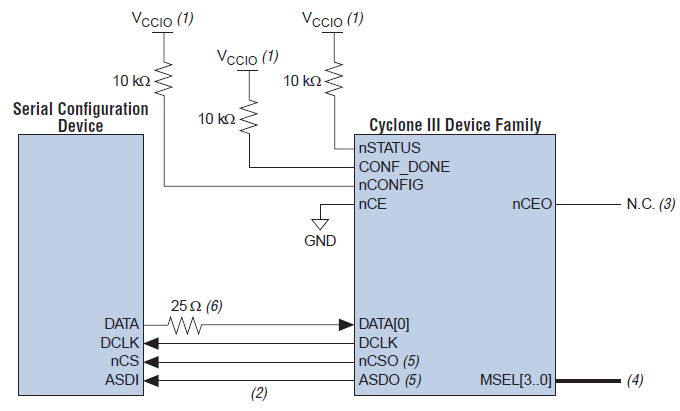
\includegraphics[width=0.9\textwidth]{figure2}
 \caption{Connections between Serial Configuration Device and Cyclone III FPGA. (from \citep{Altera:2011:cyclone3handbook})}
 \label{fig:b2_f2}
\end{figure}

A $25\Omega$ series resistor must be connected between the serial configuration device and
the Cyclone III device at the near end of the serial configuration device for \texttt{DATA[0]}
when configuring the Cyclone III device in the AS mode.

The $25\Omega$ resistor works to minimize the driver impedance mismatch with the board trace
and reduce the overshoot seen on the Cyclone III device input pin \texttt{DATA[0]}.

The maximum trace length between Cyclone III device and the serial configuration device must be less than $10in$. In the B2 PCB designing, only $8mm$ is used.

Cyclone III device uses a $40MHz$ internal oscillator to generate \texttt{DCLK} to controls the entire configuration cycle and provide timing for the serial interface.

By driving the \texttt{nCSO} output pin low, which connect to \texttt{nCS} pin of the configuration device,
the Cyclone III device enables the configuration device.  \texttt{DCLK} and \texttt{DATA[1]} pins are used
to read the configuration from the serial configuration device. The configuration device sends data
on \texttt{DATA} pin which connects to the \texttt{DATA[0]} pin of the Cyclone III device.

After all the configuration bits are received, Cyclone III releases the open-drain \texttt{CONF\_DONE} pin with a $10\Omega$ pull-up resistor. The
\texttt{CONF\_DONE} pin must have an external $10\Omega$ resistor for the device to initialize.


\subsubsection{Serial Configuration}

Cyclone III FPGAs are programmable logic devices used for basic logic functions,
chip-to-chip connectivity, signal processing, and embedded processing. They can
be programmed and configured by a microprocessor, JTAG port, or directly by a
serial PROM or flash.

A Spansion SPI (Serial Peripheral Interface) flash $S25FL064K$ can configure the FPGA easily at power-up \citep{Spansion:2011:appnote}.

The three stages of the configuration cycle are power-on reset, configuration, and initialization.
When the FPGA enters power-on reset (POR), it drives the \texttt{nSTATUS} signal low to indicate it is busy,
drives the \texttt{CONF\_DONE} signal low to indicate the configuration has not been completed, and tri-states all I/O pins.
All pins will be released after POR.

The \texttt{DCLK} generated by the FPGA device control the configuration data transferring.
The \texttt{CONF\_DONE} pin will be released with pulling high by an external pull-up
resistor after all configuration data is transferred to the FPGA. The FPGA enters user mode after internal initialization.

The SPI is a simple four-pin synchronous interface protocol which enables a master device and one or more slave devices to intercommunicate. Four signal wires are:
\begin{itemize}
 \item Master Out Slave In (MOSI) signal generated by the master (data to slave)
 \item Master In Slave Out (MISO) signal generated by the slave (data to master)
 \item Serial Clock (SCK) signal generated by the master to synchronize data transfers
 \item Slave Select (SS) signal generated by master to select individual slave devices (also known as Chip Select (CS) or Chip Enable (CE))
\end{itemize}


Figure \ref{fig:b2_f3} displays a simple block diagram of the connection between FPGA and SPI flash,
as well as the HSMC header and JTAG programming the SPI flash from a host PC or the main DE2 board.

\begin{figure}
 \centering
 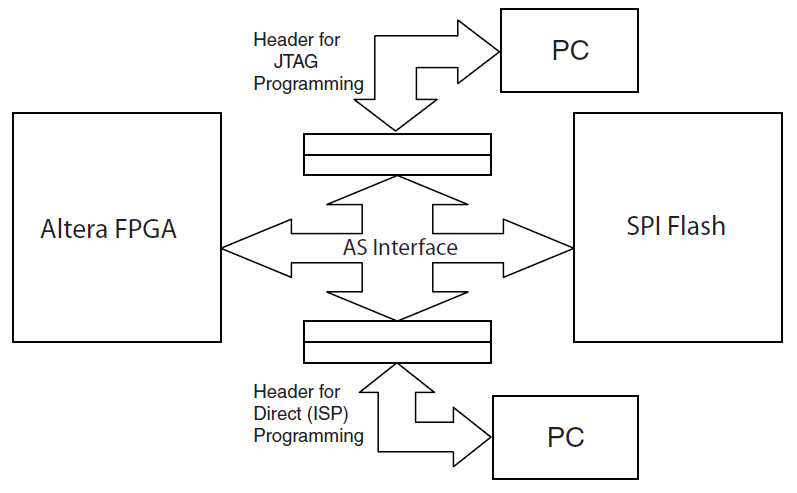
\includegraphics[width=0.9\textwidth]{figure3}
 \caption{AS interface. (from \citep{Spansion:2011:appnote})}
 \label{fig:b2_f3}
\end{figure}


Figure \ref{fig:b2_f4} displays the details of the connection between SPI flash and FPGA.

\begin{figure}
 \centering
 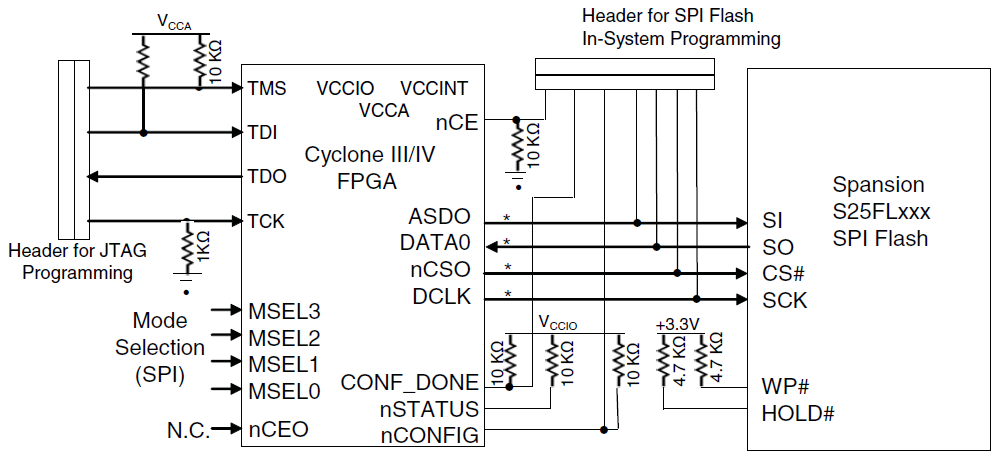
\includegraphics[width=0.9\textwidth]{figure4}
 \caption{The connection between SPI flash and FPGA in detail. (from \citep{Spansion:2011:appnote})}
 \label{fig:b2_f4}
\end{figure}

The \texttt{TMS}, \texttt{TDI}, \texttt{TDO} and \texttt{TCK} pins of Cyclone III device are
used for JTAG. The TDO pin is powered by VCCIO (3.3V). TDI and TMS are powered by VCCA (2.5V). The JTAG
scan chain on the B2 board is chained via the HSMC connector to the JTAG scan chain on the DE2 main board.


\subsubsection{External Oscillator}

As mentioned in the Cyclone III part, an external oscillator is needed as the clock source to provide a certain frequency for the FPGA.
The TXC DEL04 oscillator is a sealed clock crystal oscillator unit with high precision characteristics, which is appropriate for the FPGA.
The supply voltage range is $1.8V-5V$ \citep{TXC:osc_datasheet}.


\subsubsection{Voltage Regulator}
The B2 board needs at least three different voltage levels, as mentioned before, $VCCIO=3.3V$, $VCCINT= 1.2V$ and $VCCA=2.5V$.
The external power source is provided by the main FPGA DE2-115 board at $3.3V$. Hence two voltage regulators are used to achieve $1.2V$ and $2.5V$.

\paragraph{1.2V Voltage Regulator \texorpdfstring{$LD1117$}{LD1117}}
The $LD111712$ is a low drop voltage regulator able to provide up to $800mA$ of output current, enough to meet the
core voltage requirements as estimated by the Early Power Estimator.

Figure \ref{fig:b2_f5} is the application circuit for $1.2V$ output.

\begin{figure}
 \centering
 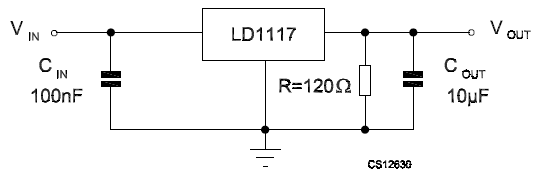
\includegraphics[width=0.9\textwidth]{figure5}
 \caption{Application circuit for 1.2V output. (from: \citep{TMicro:2012:LD1117xx})}
 \label{fig:b2_f5}
\end{figure}



\paragraph{2.5V Voltage Regulator \texorpdfstring{$TPS78225$}{TPS78225}}
The $TPS78228$ is a low dropout linear voltage regulator manufactured by TI.
The device requires minimal board space for miniaturized packaging and potentially a small output capacitor \citep{TI:2008:TPS782}.

The enable pin is active high and is compatible with standard and low-voltage CMOS levels. Therefore if the shutdown capacitor is not necessary, the enable pin can connect to the $IN$ pin as shown on figure \ref{fig:b2_f6}.

\begin{figure}
 \centering
 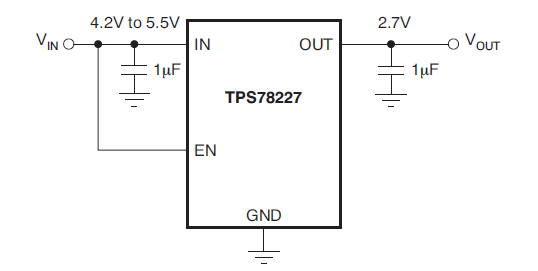
\includegraphics[width=0.9\textwidth]{figure6}
 \caption{Connection between enable and IN pins.(from \citep{TI:2008:TPS782})}
 \label{fig:b2_f6}
\end{figure}


\subsubsection{HSMC Header}
The Altera High Speed Mezzanine Card (HSMC) specification defines the electrical
and mechanical properties of the HSMC adapter interface for FPGA-based motherboards.
The HSMC connector is based on the Samtec $0.5mm$ pitch, surface-mount QTH/QSH family of connectors \citep{Altera:2009:HSMCspec}.

Two versions are used in FPGA board. $ASP-122953-01$ Socket for the host boards and $ASP-122952-01$ Header for Mezzanine Cards (slave boards).

Figure \ref{fig:b2_f7} is the diagram for HSMC header.
The JTAG and clock signals are also dedicated in Bank 1. In Banks 2 and 3, there are main CMOS/LVDS interface signals, including LVDS/CMOS clocks, as well as both $12V$ and $3.3V$ power pins.

\begin{figure}
 \centering
 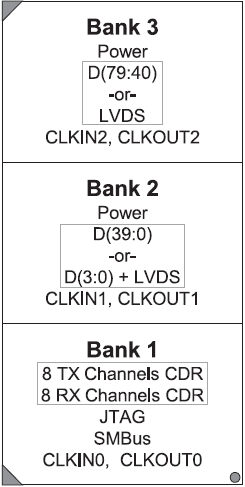
\includegraphics[width=0.3\textwidth]{figure7}
 \caption{HSMC header diagram. (from \citep{Altera:2009:HSMCspec})}
 \label{fig:b2_f7}
\end{figure}

The host board is any board with an FPGA connected to one or more HSMC interface. In this project it is the DE2-115 development board.
The interconnect I/O pins available on the HSMC connector can have all possible I/O standard and
logic features that can be supported by the host FPGA since FPGAs are configurable devices.

The HSMC connectors provide the interface between host and slave boards. The ``header''
part ($ASP-122952-01$) on slave board plugs into the ``socket'' part on the host board. The host
board provides $+12V$ DC and $+3.3V$ DC power to the slave board via the HSMC connector.
In addition to power and clock signals, the host board provides access to JTAG,
high speed serial I/O, and single-ended or differential I/O via the HSMC connector.

Figure \ref{fig:b2_f8} shows the HSMC connector diagram.

\begin{figure}
 \centering
 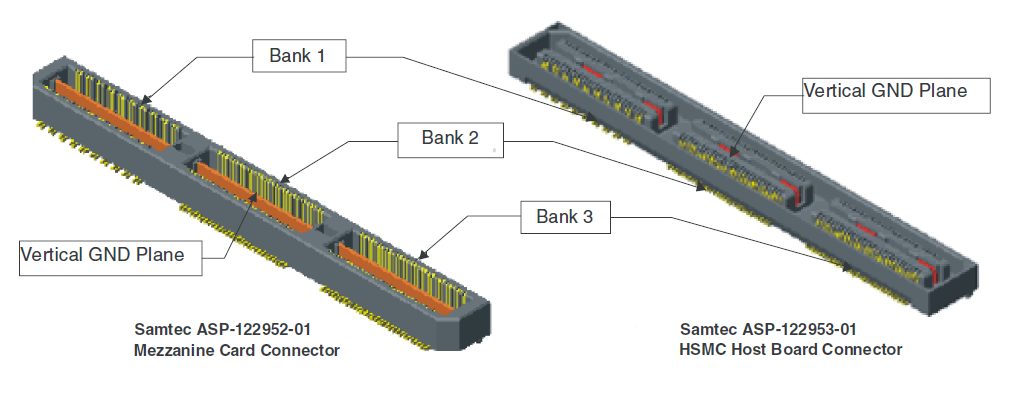
\includegraphics[width=0.9\textwidth]{figure8}
 \caption{HSMC connector modules. (from \citep{Altera:2009:HSMCspec})}
 \label{fig:b2_f8}
\end{figure}

The JTAG signals are intended to connect to dedicated JTAG pins on the host FPGA and
be part of the JTAG chain. The JTAG signals \textbf{TCK}, \textbf{TMS} and \textbf{TDI} are intended to be
output from host board while JTAG \textbf{TDO} should be the input to host board as figure \ref{fig:b2_f4} before.

Tables \ref{tab:b1_hsmc_pinout} and \ref{tab:b2_hsmc_pinout} in the appendix show the pin-outs for the HSMC header on B1 and B2 boards, respectively.












\newpage
\section{Avalon Memory Mapped Interface}
The Avalon Memory Mapped (Avalon MM) interface is used throughout the project to interconnect
blocks with memory elements and the SoPC interconnect. An example Avalon MM waveform
is shown in Figure \ref{figure:avalonmm}.
\begin{figure}[h!]
\begin{center}
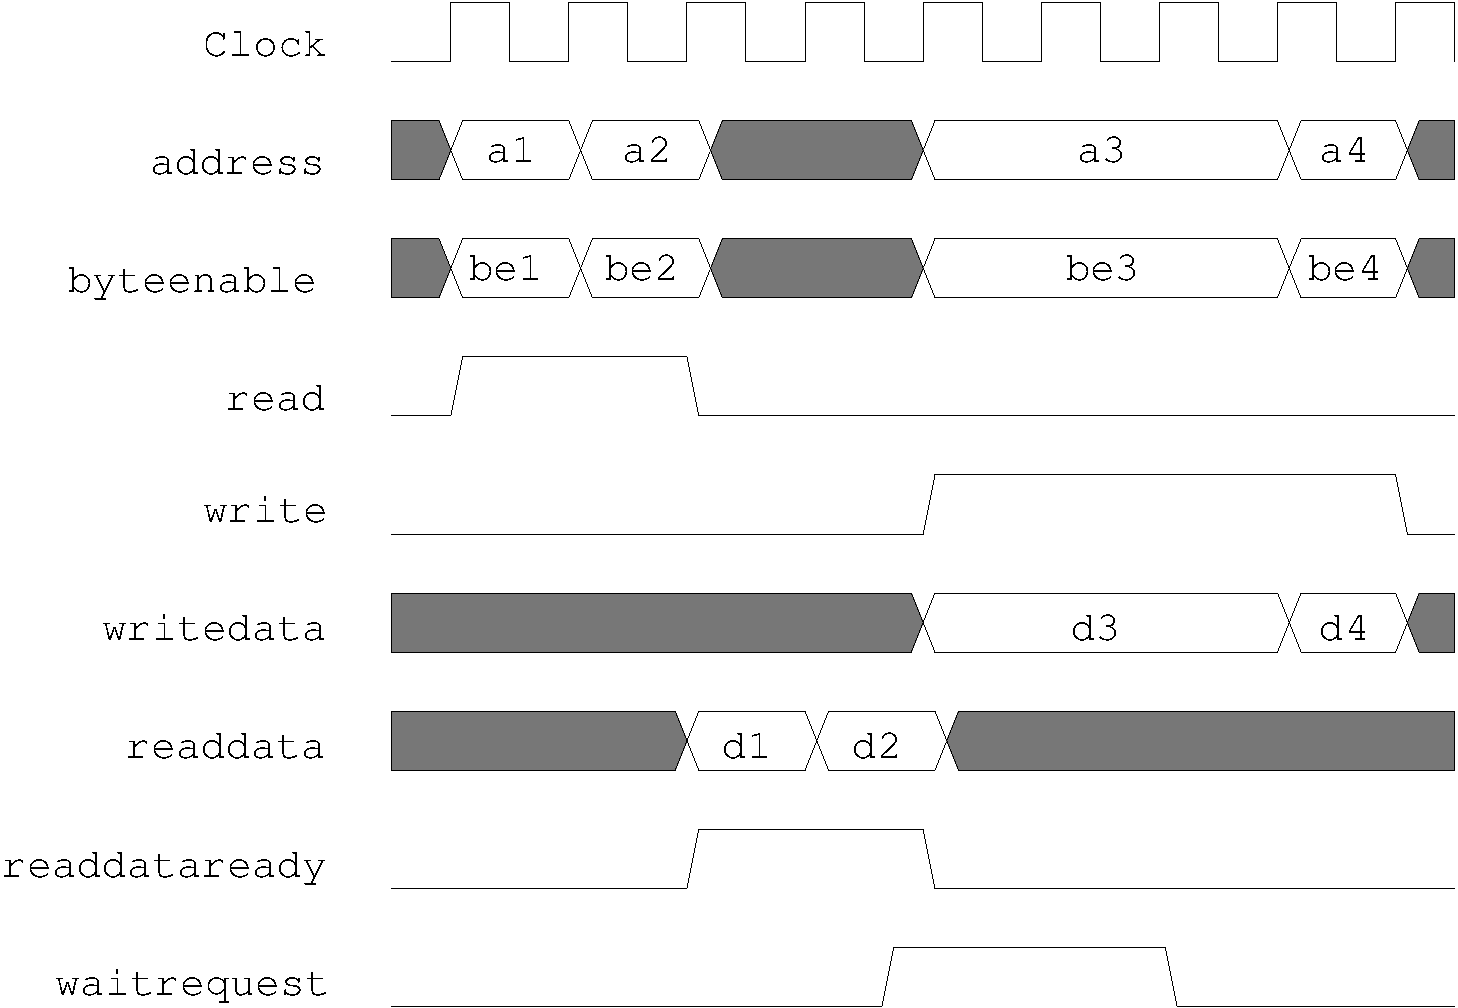
\includegraphics[width=0.95\textwidth]{avalonmm}
\caption{Example waveforms of an Avalon MM bus}
\label{figure:avalonmm}
\end{center}
\end{figure}


The master can issue both reads and writes, which a slave then replies to. A read
is initiated by setting the desired address and byte enables and asserting the \texttt{read}
signal. The master can continue issuing reads to different addresses as long as the \texttt{waitrequest}
signal stays low. If the Avalon MM slave asserts the \texttt{waitrequest} signal, the master needs
to hold the current signals for as long as the \texttt{waitrequest} signal is asserted.
The Avalon MM slave will reply to the read by asserting the \texttt{readdataready} signal
and providing the requested read data on the \texttt{readdata} bus.

Similarly writes are initiated by the Avalon MM master by setting the desired address, byte enables,
data to write and asserting the \texttt{write} signal. The master can assume that the write completed
without waiting any further unless the \texttt{waitrequest} signal is asserted, in which case,
similarly to the reads, the master needs to hold the signals steady until \texttt{waitrequest} is deasserted.



\newpage
\section{FPGA Hardware Overview}

The FPGA hardware part consists of two main blocks: the Nios II SoPC and the Tester module.

\begin{figure}
 \centering
 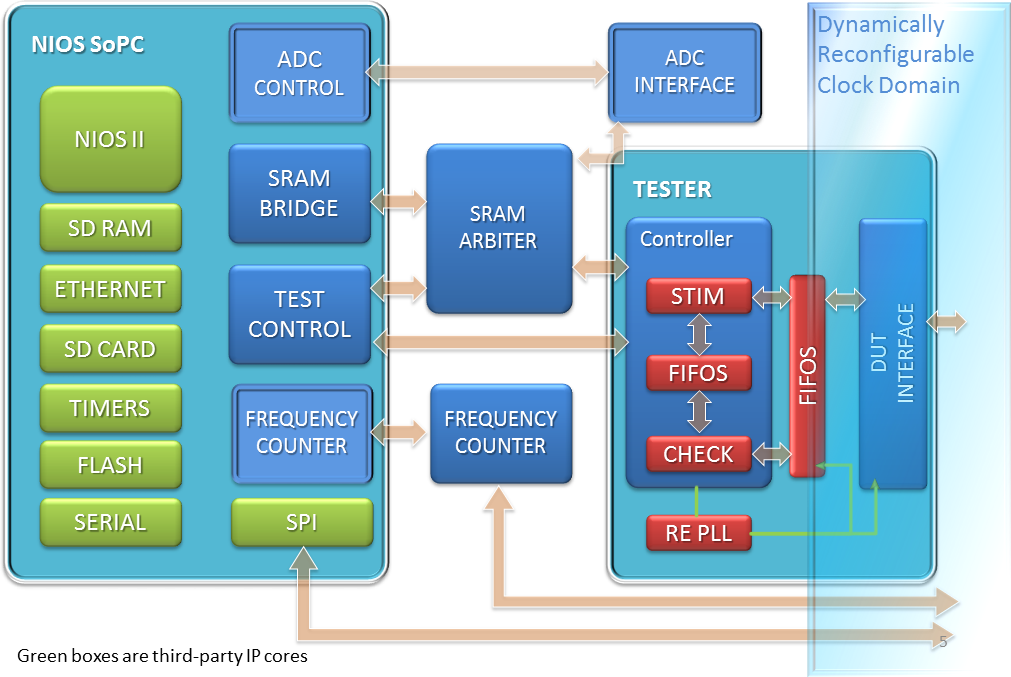
\includegraphics[width=0.9\textwidth]{hw_overview}
 \caption{Hardware Overview.}
 \label{fig:hw_overview}
\end{figure}



The \textit{Nios II SoPC} coordinates the whole system, reading and parsing the data from the SD Card
into the SRAM for the Tester to read the data from it; retrieving the result that the
Tester writes back to the SRAM and sending the data to the backend for archiving and reviewing from the users.

Its tasks include:
\begin{itemize}
 \item coordinating the data from multiple sources (SRAM, SD Card, Flash, Serial connection, SPI bus, Ethernet, etc.)
 \item controlling the testing process (which is executed by the Tester, frequency counter and ADC)
 \item sending results to the backend
\end{itemize}

The \textit{SRAM arbiter} provides arbitrated access to the on-board SRAM to the SoPC, tester module and ADC module via
an Avalon Memory Mapped Interface (Avalon-MM). It translates the Avalon-MM requests by the different modules into
the signals needed by the asynchronous SRAM.

The \textit{Tester} contains several HDL blocks which are responsible for the testing process:
\begin{itemize}
 \item read the command, request and test vector from SRAM
 \item generate the test input signals for every pin of the DUT
 \item monitor the output pins of the DUT and write the result into the memory when it is valid
 \item offer a dynamically reconfigurable clock for the DUT and its relative interface
\end{itemize}

The purpose of the \textit{frequency counter} and the \textit{ADC} is that there is a designated
pin on the chip under test which is the output of a ring oscillator. It is preferable that not only
the frequency of this clock output is tested, but that the output waveform is also monitored.


\newpage
\section{Tester}
The tester module is responsible for applying test vectors to the device under test, as well as
reading and checking the results. Figure \ref{fig:tester} shows an overview.

\begin{figure}
 \centering
 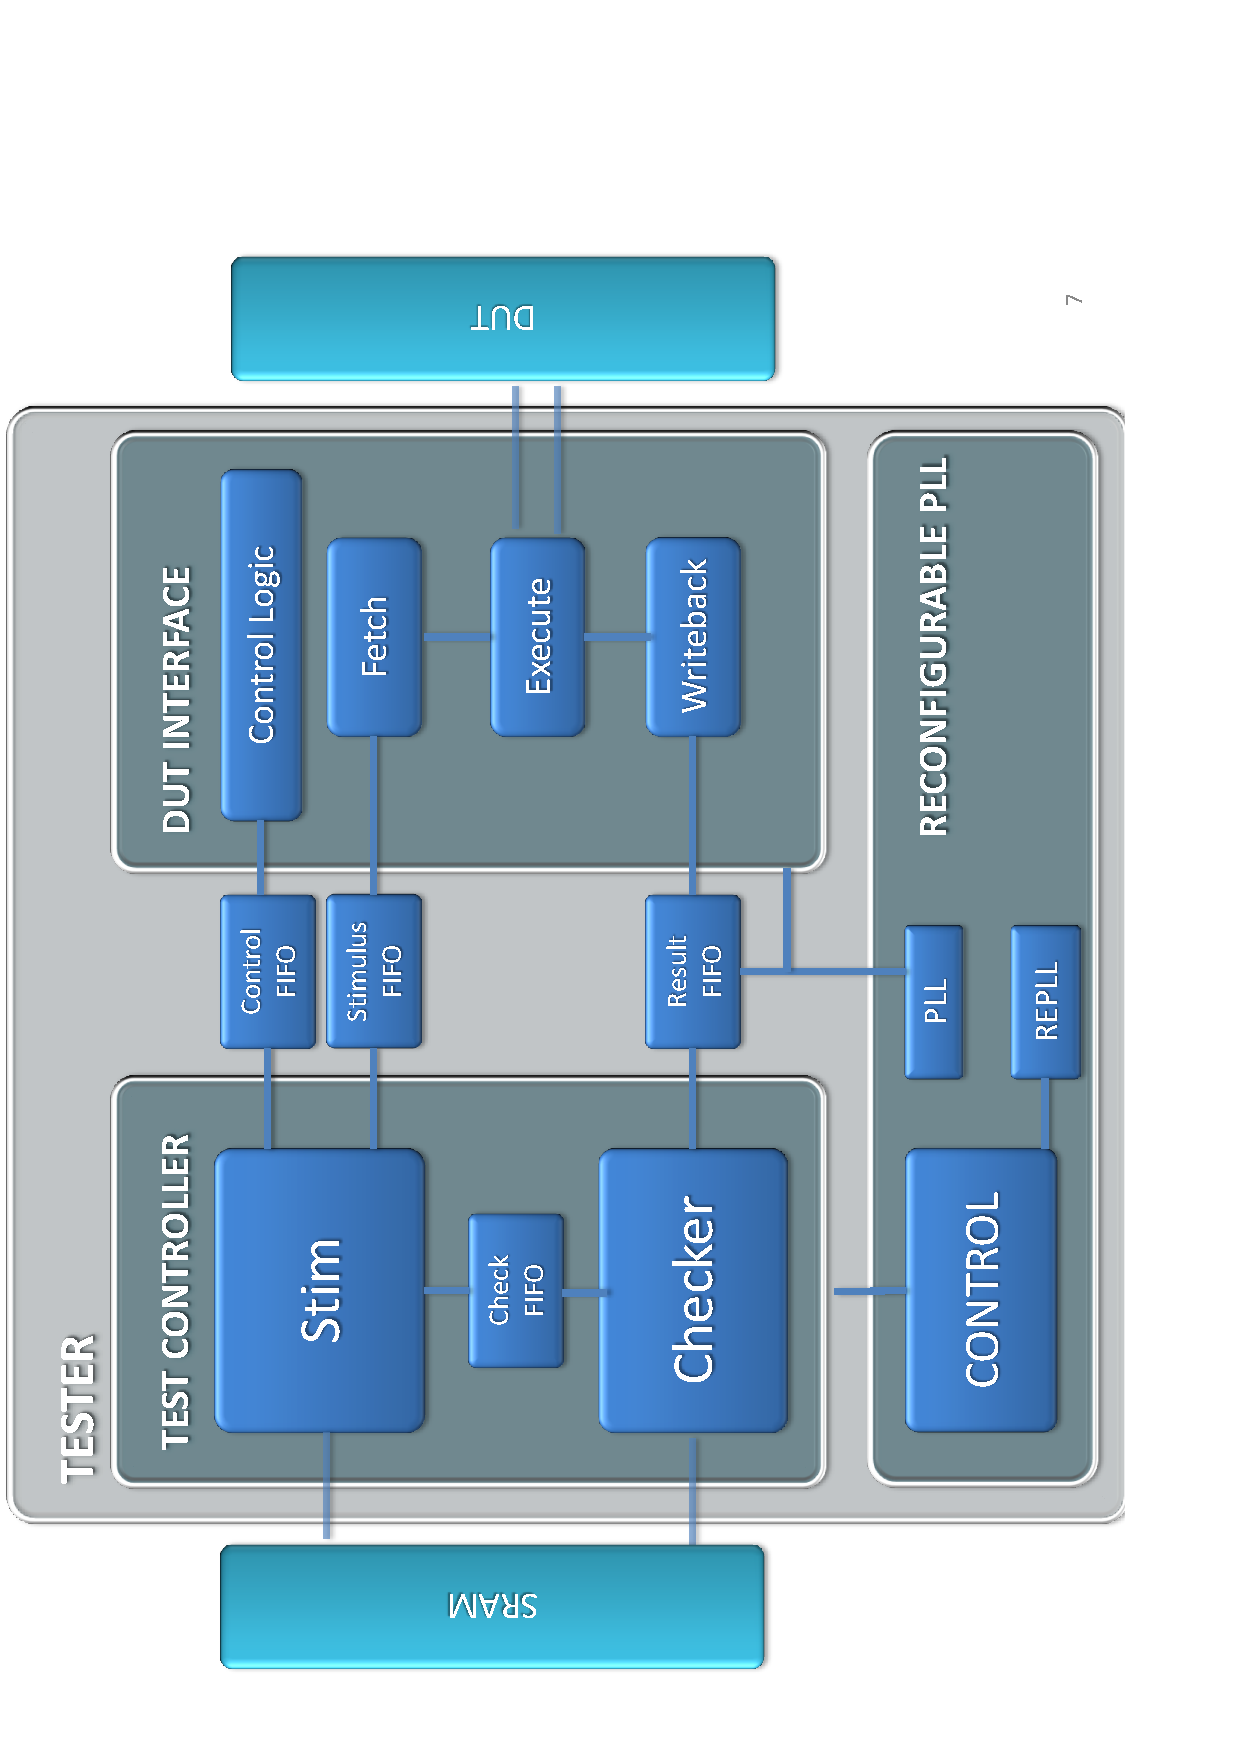
\includegraphics[width=0.8\textwidth,angle=270]{tester}
 \caption{More detailed view of the tester module.}
 \label{fig:tester}
\end{figure}

The \textbf{test\_controller} module reads test vectors and commands from the SRAM. It also controls
the reconfigurable PLL and provides test vectors to the actual DUT interface module \textbf{dut\_if}.

The \textbf{dut\_if} module applies the test vectors to the device under test and reads back the results.
The results are sent back to the \textbf{test\_controller}, which then compares the result with the
expected result and writes back the final result to SRAM.

Figure \ref{fig:bb_tester} shows a black box view of the tester module. It uses an Avalon MM interface
to interface with the SRAM via the SRAM Arbiter described in a later section. The \texttt{enable} and \texttt{done}
signals are used to interface with a module within the SoPC that controls the tester.

The \textbf{tester} module also has the interface to the DUT (device under test), including outputs, inputs and the target select.

\begin{figure}
 \centering
 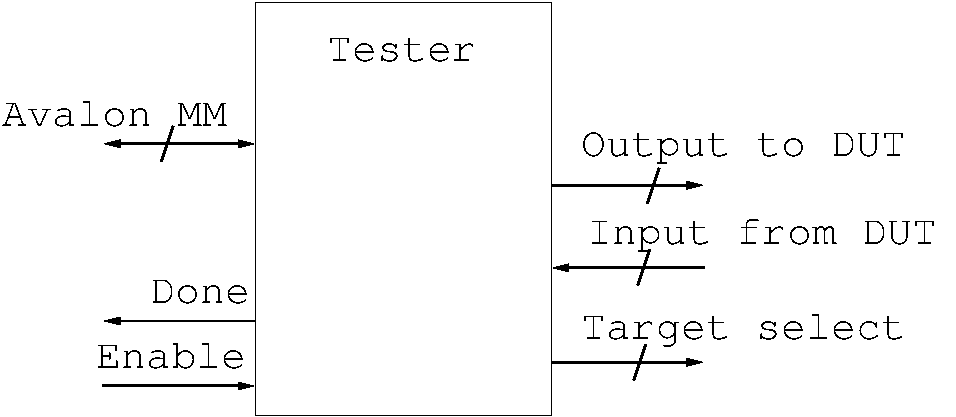
\includegraphics[width=0.4\textwidth]{tester_bb}
 \caption{Black box view of the tester}
 \label{fig:bb_tester}
\end{figure}


The design under test (DUT) is isolated from the clock domain of the main board,
since various designs may operate on different clock frequencies. In order to realize this,
a dynamically reconfigurable Phase Lock Loop (PLL) was used.

As a result of having two clock domains and to ensure data integrity between them Dual-Clock First-In-First-Out (DCFIFO) with synchronizer megafunctions were used,
In the DCFIFO, the read and write signals are synchronized to the \texttt{rdclk} and \texttt{wrclk} clocks respectively.
When the \texttt{wrfull} signal is low, asserting \texttt{wrreq} writes the data
on the data lines into the FIFO.
When the \texttt{rdempty} port is low, asserting \texttt{rdreq} issues a read request.
Then the data will be output on the \texttt{q} port.
The \texttt{aclr} signal is used for clearing the data stored in the DCFIFO.

%%The figure below shows the timing and behaviour of the write and read process.

%XXX: MISSING FIGURE???



\subsection{Test Controller}
Figure \ref{fig:bb_test_controller} shows a black box view of the test controller. The Avalon MM bus and
\texttt{enable} and \texttt{done} signals from the \textbf{tester} module are fed through
to the \textbf{test\_controller}.

It also contains control outputs to both the \textbf{dut\_if} and reconfigurable PLL, as well as the actual
test vector output and result input to/from the \textbf{dut\_if}.

\begin{figure}
 \centering
 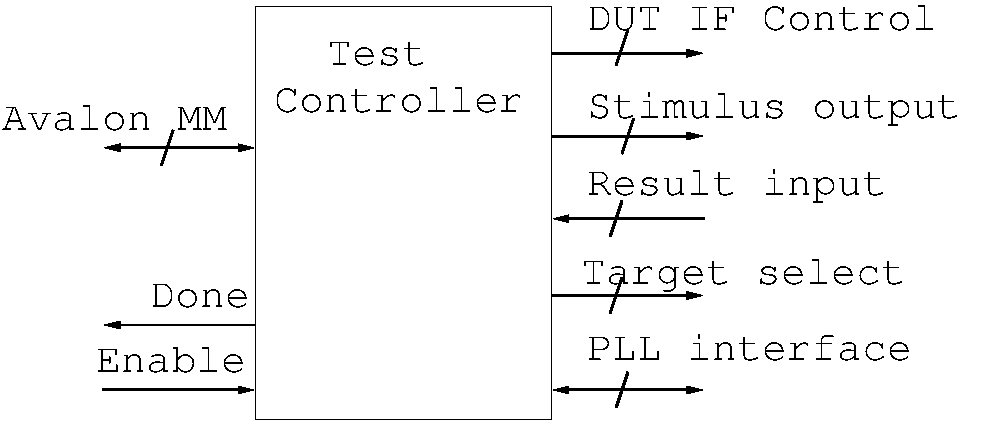
\includegraphics[width=0.4\textwidth]{test_controller}
 \caption{Black box view of the test controller}
 \label{fig:bb_test_controller}
\end{figure}



\subsubsection{mem\textunderscore if}
The \textbf{mem\_if} module, not shown in Figure \ref{fig:tester}, arbitrates the memory access to the SRAM arbiter (and hence to the SRAM)
 between the \textbf{stim} and \textbf{check} module. Figure \ref{fig:bb_mem_if} shows a black box view. It has
an Avalon MM interface to the main SRAM arbiter, and two Avalon MM interfaces to the \textbf{stim} and
\textbf{check} modules. Arbitration is done in a read-before-write fashion, so that the arbitration is always
in favour of the \textbf{stim} module.

\begin{figure}
 \centering
 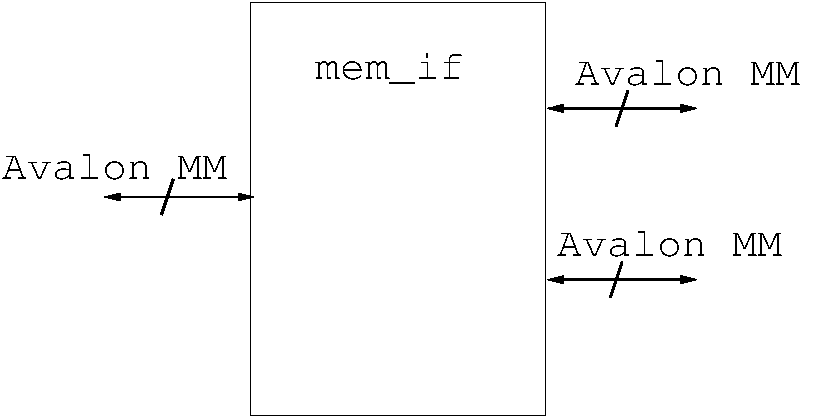
\includegraphics[width=0.4\textwidth]{mem_if}
 \caption{Black box view of the mem\_if module}
 \label{fig:bb_mem_if}
\end{figure}



\subsubsection{stim}
The \textbf{stim} module is the main part of the controller. It reads requests written by the SoPC to the SRAM and
processes them either into test vectors or local configuration commands. Figure \ref{fig:bb_stim} shows a black box
view of the \textbf{stim} module.

\begin{figure}
 \centering
 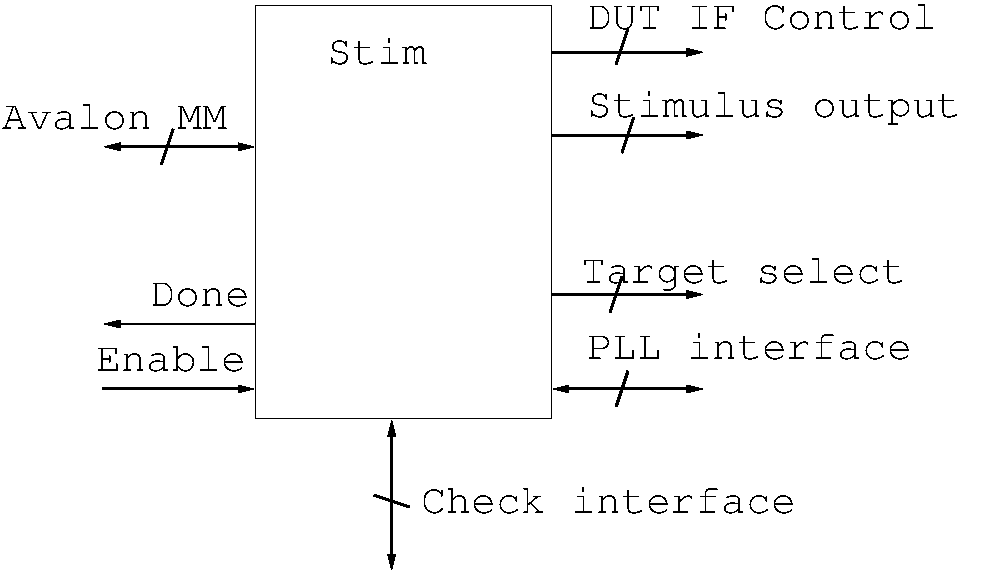
\includegraphics[width=0.4\textwidth]{stim}
 \caption{Black box view of stim module}
 \label{fig:bb_stim}
\end{figure}



Figures \ref{fig:req_test_vector}, \ref{fig:req_change_bitmask},
\ref{fig:req_change_target}, \ref{fig:req_pll_reconfig}, \ref{fig:req_send_dicmd}, \ref{fig:req_metadata} and \ref{fig:req_metadata_2}
show the format of the requests understood by the \textbf{stim} module.

All requests have a metadata field at the beginning. The main content of the metadata field are the first three bits
which define the request type and are used by the \textbf{stim} module to determine which request is being processed.
All requests are padded to be at least 3 words long to hide the latency of the \textbf{sram\_arb\_sync} pipeline described
later.

\begin{figure}[h]
 \centering
 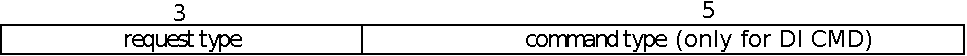
\includegraphics[width=0.9\textwidth]{metadata}
 \caption{Metadata.}
 \label{fig:req_metadata}
\end{figure}

The \texttt{test\_vector} request contains a standard test vector. After the metadata there are 24 bits of input, making up
the input vector applied to the DUT. This is followed by 24 bits of the expected result and a metadata2 field made up of
several fields shown in figure \ref{fig:req_metadata_2}. The metadata2 carries information on whether a test passed or failed,
whether it has been run, whether a trigger-type test has timed out and a count of how long it took to execute.
The timeout flag serves a double purpose: when the vector is first read, it defines whether a test
is a fixed latency or variable latency (triggered) test. After the test has run, it serves to indicate whether the test has timed out or not.

Similarly the cycle count is used as an input initially, containing the cycle count for a fixed latency test and the maximum cycle
count that a triggered test can take.

These metadata2 fields are extracted and, alongside the input vector itself, are passed to the DUT interface over the stimulus FIFO.
The expected result (output vector) is written to the check FIFO for use by the \textbf{check} module.

The metadata2 field is followed by 24 bits of a don't care mask. This don't care mask is used in the \textbf{check} module to
mask off bits. This field is generated from the 'X' entries in a vector configuration line in the configuration files. This don't care
mask is also passed through the check FIFO to the \textbf{check} module.

Test vectors are continuously written to the FIFOs until the FIFOs are full. If the FIFOs fill up, the module will idle
until there is enough space to continue.

\begin{figure}[h]
 \centering
 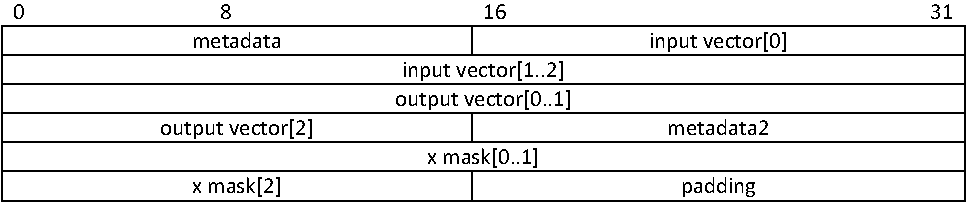
\includegraphics[width=0.9\textwidth]{test_vector}
 \caption{Test Vector.}
 \label{fig:req_test_vector}
\end{figure}

\begin{figure}[h]
 \centering
 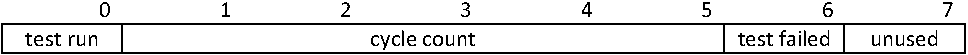
\includegraphics[width=0.9\textwidth]{metadata_2}
 \caption{Metadata 2.}
 \label{fig:req_metadata_2}
\end{figure}


The change target request (Figure \ref{fig:req_change_target}) is generated by the software when the target needs to be switched
from one design on the chip to another. The \textbf{stim} module will wait for all FIFOs to drain before starting a target switch.
After a target switch the module will wait for a number of clock cycles to make sure the external DUT has time to power up.

\begin{figure}[h]
 \centering
 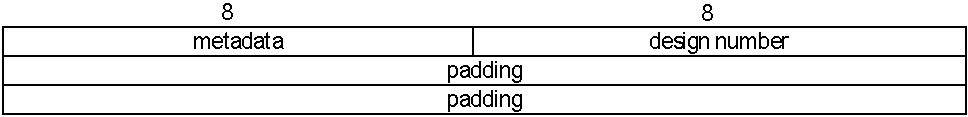
\includegraphics[width=0.9\textwidth]{change_target}
 \caption{Change Target.}
 \label{fig:req_change_target}
\end{figure}


The change bitmask request shown in Figure \ref{fig:req_change_bitmask} is generated by the ``pindef'' line in the configuration.
In addition to the don't care mask in each vector, this defines the bits of the output and expected result that are not of
interest when comparing them.

\begin{figure}[h]
 \centering
 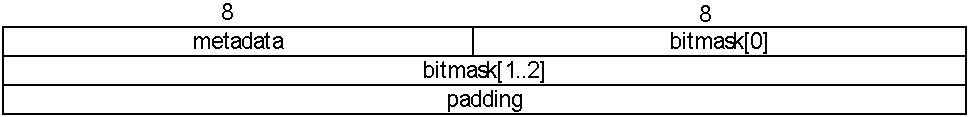
\includegraphics[width=0.9\textwidth]{change_bitmask}
 \caption{Change Bitmask.}
 \label{fig:req_change_bitmask}
\end{figure}


The send DICMD request in Figure \ref{fig:req_send_dicmd} is used to pass arbitrary messages to the \textbf{dut\_if} module. The
type of the message is contained in the metadata as shown in Figure \ref{fig:req_metadata}. The payload content depends on the
message type. The two currently defined commands are:
\begin{itemize}
 \item \texttt{DICMD\_SETUP\_MUXES} - the payload contains a bitmask of which of the input pins to the DUT are connected to the normal
input vector and which ones are instead connected to the dut clock.
 \item \texttt{DICMD\_TRGMASK} - the payload contains information on which pins the triggering tests trigger on. A 1 in the payload means that the bit at that
position of the output of the DUT needs to be 1 for a triggered test to be triggered.
\end{itemize}

\begin{figure}[h]
 \centering
 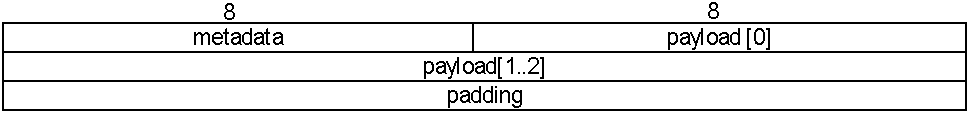
\includegraphics[width=0.9\textwidth]{send_dicmd}
 \caption{Send dicmd.}
 \label{fig:req_send_dicmd}
\end{figure}


The PLL reconfiguration request in Figure \ref{fig:req_pll_reconfig} is used to reconfigure the frequency
of the dynamic PLL. The request contains the loop multiplier and divider factors as well as the
post-scale counter. This information is passed to the PLL reconfiguration module.

\begin{figure}[h]
 \centering
 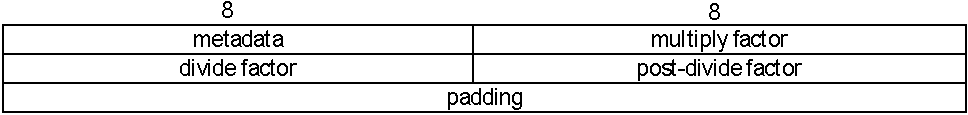
\includegraphics[width=0.9\textwidth]{pll_reconfig}
 \caption{PLL Reconfiguration.}
 \label{fig:req_pll_reconfig}
\end{figure}


The mem end request defines the end of the used memory. A mem end request will cause the \textbf{stim} module
to wait for all FIFOs to drain before becoming idle.
\begin{figure}[h]
 \centering
 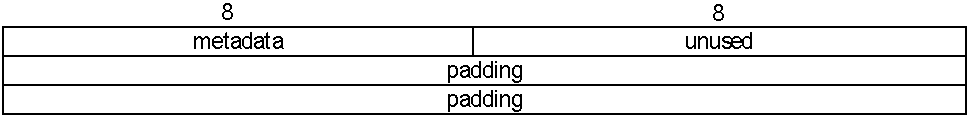
\includegraphics[width=0.9\textwidth]{mem_end}
 \caption{Mem End.}
 \label{fig:req_mem_end}
\end{figure}



The request types are read in the \texttt{READ\_META} state. Depending on the request type, the state machine will transition to
one of \texttt{READ\_TV}, \texttt{SEND\_DICMD}, \texttt{SETUP\_BITMASK}, \texttt{START\_REPLL} or \texttt{SWITCH\_TARGET}.

The action taken for each request type is outlined below:
\begin{itemize}
 \item setup bit mask (SETUP\_BITMASK). In this task the bit mask and relative command type are sent to the \textbf{check} module through a register output, bypassing the FIFO between \textbf{stim} and \textbf{check}.

 \item read test vector (READ\_TV, WR\_FIFOS). The test vector is firstly read from memory in serial, then sent to the \textbf{dut\_if} for the input of the design and to the \textbf{check} for reference through FIFOs in this task.

 \item send command/data to \textbf{dut\_if} (SEND\_DICMD, WR\_DIFIFO). This task is used for assigning clock pins to the DUT inputs and setting up trigger pins to the DUT output pins. These are explained in the \textbf{dut\_if} section.

 \item switch design target (SWITCH\_TARGET, SWITCH\_VDD). As introduced previously, there are 16 designs at most on a single chip under test. Only one can be selected by powering up its exclusive VDD pin. In this task, a $4-bit$ signal indicating which design is selected is sent to the testing board. On the B1 board, a $4-16$ decoder will decode the information and the integrated switches array will turn on only one design.

 \item start reconfiguring the dynamic PLL (START\_REPLL, PLL\_RECONFIG, PLL\_WAIT). In this task, the parameters for the PLL counters are read from the memory first. Then in the PLL\_RECONFIG state a trigger will be sent to the PLL\_INTERFACE module with those parameters to start the configuration process. Then the PLL\_WAIT state will halt the ``stim'' until the new PLL output frequency is stable.
\end{itemize}

After each task is done, the \textbf{stim} returns to the IDLE state, waiting for the next request. When a complete test is finished, the \textbf{stim} goes to an END state and resets itself to the start IDLE state.

The detailed state transition chart is shown in figure \ref{fig:hw_state_trans_chart}. Table \ref{tab:states_behaviour} contains a more detailed
explanation of what occurs in which state, while Table \ref{tab:states_transitions} contains all the state transition conditions.


\begin{figure}
 \centering
 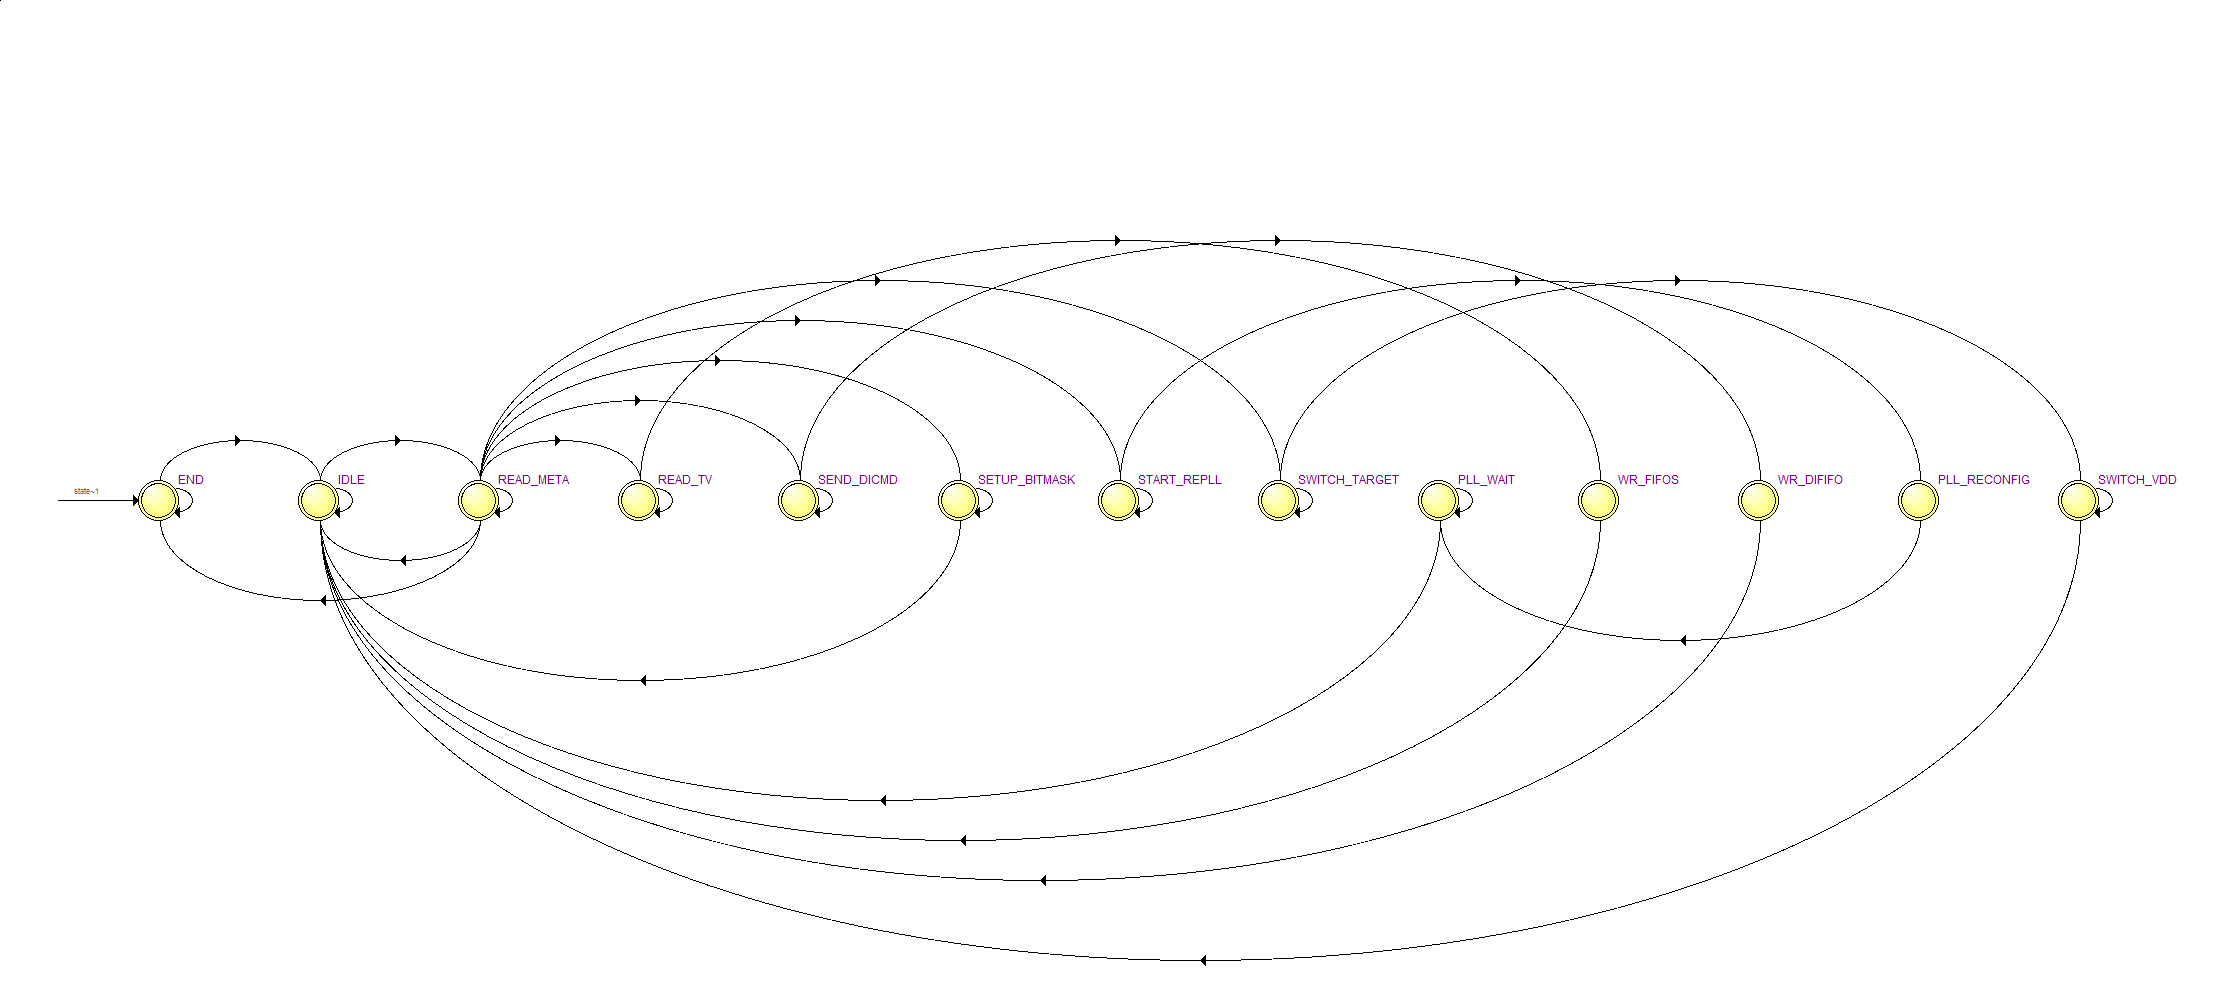
\includegraphics[width=0.9\textwidth]{hw_state_trans_chart}
 \caption{State Transition Chart.}
 \label{fig:hw_state_trans_chart}
\end{figure}

\begin{table}[ht]
\centering
\begin{tabular}{|l|p{0.5\textwidth}|}
\hline
State & Behaviour \\
\hline
\texttt{IDLE} & reset variables (\texttt{words\_stored}, \texttt{read\_requested}) \\
\texttt{READ\_META} & read metadata from memory \\
\texttt{READ\_TV} & read test vector from memory \\
\texttt{SWITCH\_TARGET} & waits until all FIFOS are drained, read target information from memory and store in \texttt{new\_target\_sel} \\
\texttt{SWITCH\_VDD} & change target power based on the \texttt{target\_sel} data (updated by \texttt{new\_target\_sel}) \\
\texttt{WR\_FIFOS} & send write request to FIFOs by \texttt{sfifo\_wrreq}, \texttt{cfifo\_wrreq} (effectively sending an input vector and expected result) \\
\texttt{SETUP\_BITMASK} & read bitmask from memory, send \texttt{sc\_cmd}, \texttt{sc\_data} to check module \\
\texttt{SEND\_DICMD} & read command data for \textbf{dut\_if} \\
\texttt{WR\_DIFIFO} & send write request to \textbf{dut\_if} through dififo \\
\texttt{START\_REPLL} & read data for PLL reconfiguration from memory \\
\texttt{PLL\_RECONFIG} & send trigger to PLL to start the reconfiguration process \\
\texttt{PLL\_WAIT} & put the \textbf{stim} waiting until the PLL clock is stable \\
\texttt{END} & when all the FIFOs are empty, send done signal to upper level \\
\hline
\end{tabular}
\caption{States Behaviour Table.}
\label{tab:states_behaviour}
\end{table}

\begin{table}[ht]
\centering
\begin{tabular}{|l|l|p{0.45\textwidth}|}
\hline
Source State & Destination State & Condition \\
\hline
\texttt{END} & \texttt{IDLE} & \texttt{sfifo\_wrempty} \&\& \texttt{cfifo\_wrempty} \&\& \texttt{enable} \\
\hline
\texttt{IDLE} & \texttt{READ\_META} & \texttt{$\sim$sfifo\_wrfull} \&\& \texttt{$\sim$cfifo\_wrfull} \&\& \texttt{$\sim$mem\_waitrequest} \\
\hline
\texttt{READ\_META} & \texttt{END} & \texttt{words\_stored} \&\& \texttt{req\_type} == \texttt{REQ\_END} \\
\hline
\texttt{READ\_META} & \texttt{IDLE} & \texttt{words\_stored} \&\& \texttt{req\_type} == \texttt{REQ\_PLLRECONFIG} \\
\hline
\texttt{READ\_META} & \texttt{READ\_META} &  \\
\hline
\texttt{READ\_META} & \texttt{SWITCH\_TARGET} & \texttt{words\_stored} \&\& \texttt{req\_type} == \texttt{REQ\_SWITCH\_TARGET} \\
\hline
\texttt{READ\_META} & \texttt{READ\_TV} & \texttt{words\_stored} \&\& \texttt{req\_type} == \texttt{REQ\_TEST\_VECTOR} \\
\hline
\texttt{READ\_META} & \texttt{SEND\_DICMD} & \texttt{words\_stored} \&\& req\_type == \texttt{REQ\_SEND\_DICMD} \\
\hline
\texttt{READ\_META} & \texttt{SETUP\_BITMASK} & \texttt{words\_stored} \&\& req\_type == \texttt{REQ\_SETUP\_BITMASK} \\
\hline
\texttt{READ\_TV} & \texttt{WR\_FIFOS} & \texttt{words\_stored} == 6 \\
\hline
\texttt{SEND\_DICMD} & \texttt{WR\_DIFIFO} & \texttt{words\_stored} == 3 \&\& \texttt{$\sim$dififo\_wrfull} \&\& \texttt{sfifo\_wrempty} \&\& \texttt{cfifo\_wrempty} \\
\hline
\texttt{SETUP\_BITMASK} & \texttt{IDLE} & \texttt{words\_stored} == 3 \\
\hline
\texttt{START\_REPLL} & \texttt{PLL\_RECONFIG} & \texttt{words\_stored} == 3 \&\& \texttt{pll\_locked} \\
\hline
\texttt{PLL\_RECONFIG} & \texttt{PLL\_WAIT} &  \\
\hline
\texttt{PLL\_WAIT} & \texttt{IDLE} & \texttt{pll\_stable} \\
\hline
\texttt{SWITCH\_TARGET} & \texttt{SWITCH\_VDD} & \texttt{sfifo\_wrempty} \&\& \texttt{cfifo\_wrempty} \\
\hline
\texttt{SWITCH\_VDD} & \texttt{IDLE} & \texttt{waitcnt} == 0 \\
\hline
\texttt{WR\_DIFIFO} & \texttt{IDLE} &  \\
\hline
\texttt{WR\_FIFOS} & \texttt{IDLE} &  \\
\hline
\end{tabular}
\caption{Main States Transitions Table.}
\label{tab:states_transitions}
\end{table}






\subsection{check}
Figure \ref{fig:bb_check} shows a black box view of the \textbf{check} module.
The check module is responsible for checking the results provided by the DUT interface
in response to a test vector with the expected result for that test vector.

\begin{figure}
 \centering
 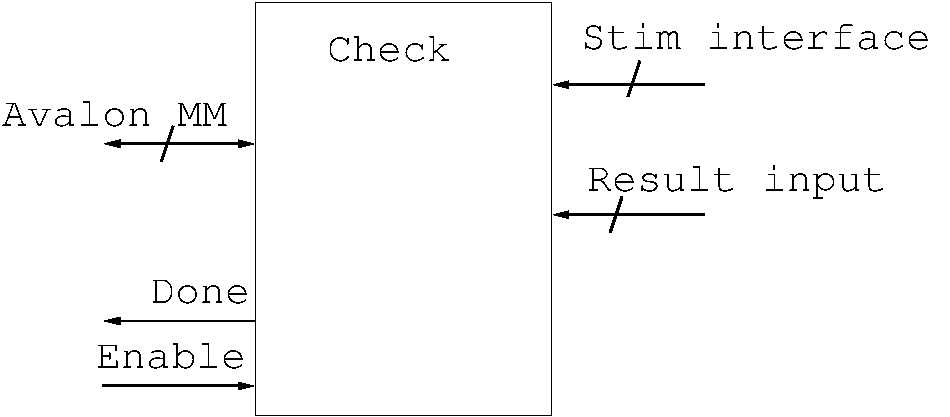
\includegraphics[width=0.4\textwidth]{check}
 \caption{Black box view of check module}
 \label{fig:bb_check}
\end{figure}


Thanks to the use of FIFOs for both the expected result and actual result, the
\textbf{check} module can simply read from both FIFOs when they are not empty and
the data will match up, as everything happens in order, even though events occur
across different clock domains. In other words the first word to be read from the
check FIFO will match up with the first word read from the result FIFO, greatly
simplifying the logic.

The \textbf{check} module operates when both the check FIFO and the result FIFO aren't
empty. It first transitions to a \texttt{READ\_FIFO} state during which a word
is read from each of the FIFOs. In the next state, \texttt{CMP\_AND\_MASK}, the
returned result from the FIFOs is masked according to the bitmask and the don't care
mask, then compared. This comparison sets the fail flag in the \texttt{metadata2}.

The \texttt{run} flag is always set at this stage. Other information in \texttt{metadata2}
is taken directly from information provided via the result FIFO from the \texttt{dut\_if}.

The actual result and the changed metadata2 are written back to memory during the next state,
\texttt{WRITEBACK}. If the memory is currently busy (as indicated by the waitrequest flag)
because the \textbf{stim} module is currently reading, the \texttt{WRITEBACK} is delayed.

\subsubsection{Test throughput}
The sustained throughput is limited by the SRAM bandwidth, the number of words read by
the \texttt{stim} module and the number of words written back by the \texttt{check} module.

The request formats have been carefully chosen so as to minimize the amount of cycles
needed for the reads and writes. A writeback for a test for example only takes up two cycles.

A test vector read takes 6 cycles to read, one cycle to write to the FIFOs and one
cycle to determine the request type. The writeback from \texttt{check} can occur in the shadow of the FIFO write
and request type determination. Hence the maximum sustained throughput is 12.5 million tests per second, or
effectively a test frequency of 12.5 MHz.

If the DUT domain frequency is lower than this, the FIFOs at the interface between the controller and the
DUT interface will fill up and the controller will stall. If on the other hand the frequency is higher, the FIFOs
will drain and the DUT interface will stall.



\subsubsection{dut\textunderscore if}
Figure \ref{fig:bb_dut_if} shows the blackbox view of the \textbf{dut\_if} module. It connects via a command FIFO, stimulus FIFO
and result FIFO to the \textbf{test\_controller}. It connects to the DUT via an input and an output bus.


\begin{figure}
 \centering
 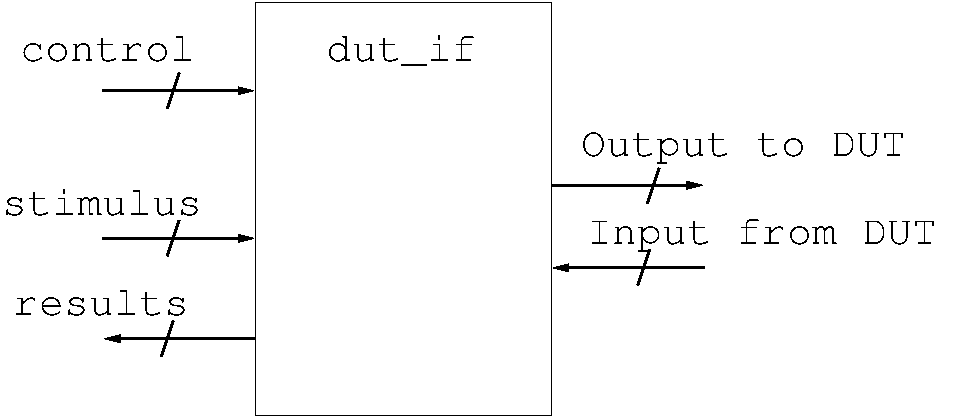
\includegraphics[width=0.4\textwidth]{dut_if}
 \caption{Black box view of dut\_if module}
 \label{fig:bb_dut_if}
\end{figure}


The \textbf{dut\_if} module is the interface between the test controller and the design under test (DUT).
It uses the data from \textbf{stim} to generate the test vector and send it to the DUT. Each of the inputs
to the DUT has a multiplexer which, depending on a register in the DUT interface will either connect the
input to the reconfigurable clock or to the actual input vector as provided by the \textbf{stim} module.

The value of this register can be modified by using a DICMD as explained in the \textbf{stim} module section.

Since it is possible for the \textbf{dut\_if} to stall when the frequency is higher than the maximum sustained
test throughput, the clock connected to the input pins of the DUT is gated. This way the clock is effectively
disconnected when no new input vectors are available.

For maximum throughput the \textbf{dut\_if} module uses a pipelined design. The pipeline consists of three stages
as shown in figure \ref{fig:tester}. During the \texttt{FETCH} stage, the stimulus FIFO is read. During the \texttt{EXECUTE}
stage the input vector is applied to the output multiplexers and hence to the DUT inputs. In the case of a 1-cycle
fixed latency test, the next cycle will take place in the next pipeline stage, \texttt{WRITEBACK}, which writes the result
received from the DUT back to the result FIFO which is then later read by the \textbf{check} module.

However, the \texttt{EXECUTE} stage can take longer than one cycle to run. In this case, a pipeline bubble is inserted forward
and a stall is signaled to the \texttt{FETCH} stage. This is the case when the test takes longer than one cycle to run, which
is the case for triggered tests and for fixed latency tests with a greater than one cycle count.
In deciding whether the result is valid, the ``dut\_if'' supports two modes.

\begin{enumerate}
 \item With a predefined clock cycle number (in metadata), the dut\_if sets up a counter to wait until the clock cycles are reached. Then the result is considered valid. If the clock cycle number is 0, the result is taken within the same clock cycle, which corresponds to a combinational logic circuit. Otherwise, the DUT should be a sequential design with a fixed clock cycle to output the valid result.

 \item With a set of pins which is defined as the trigger (e.g. a \texttt{done} or \texttt{ready} signal). The result is considered valid when the triggers change. This corresponds to asynchronous handshake behaviour. This is implemented by the trigger mask.
\end{enumerate}

Those different modes of operation are set by the user in the metadata, depending on specific designs.

In the case of triggered
tests, the \texttt{EXECUTE} stage will stall until the result from the DUT matches the trigger mask as passed in from the
\textbf{stim} module via an earlier DICMD. In the case of fixed latency tests, a counter increases every clock cycle and once
that counter matches the wanted cycle count stored in the input vector provided by the \textbf{stim} module, the pipeline
will unstall and continue operation. This same counter is also used to provide a timeout for triggered tests and in general
keep track of how long a triggered test takes, even if it is triggered before the timeout.


The speed of the \textbf{dut\_if} is boosted by pipelining technique, including fetch, execute and writeback stages. The fetch stage checks whether the \textbf{sfifo} is empty and decide if the process should go to the next stage.
The effective throughput of the \textbf{dut\_if} module without considering the limitations of the \textbf{test\_controller} described earlier is one test per cycle for 1-cycle tests.

\subsubsection{PLL INTERFACE}
The reconfigurable clock domain uses the Altera IP cores ALTPLL and
\\
ALTPLL\_RECONFIG to realize the dynamically reconfigurable clock.
The ALTPLL generates stable clock. The input clock frequency is divided and multiplied by the internal counters,
resulting in a variable output frequency. The parameters are initialized by a scan chain.
Reinitializing the PLL with a new scan chain is possible and can change the output frequency with different parameters.
However the scan chain contains too much information that is not expected to change during the frequency reconfiguration process
(counters that are not changed, current, phase information, etc.).

The ALTPLL\_RECONFIG module can change specific parameters based on a complete scan chain and reinitialize the ALTPLL without having to provide new values for each parameter.

The ALTPLL\_RECONFIG module requires input to be in serial and specific timing requirements. The process is coordinated by REPLL\_CONTROL, responding to an input trigger, transferring the parallel input into serial, and offering a stable signal when the reconfiguration is done. All these modules are enveloped in PLL\_INTERFACE.

The counters used here are M (feedback multiplier counter), N (pre-divider counter) and C (post-divider counter) counters. The output frequency = input frequency * M/(N*C). Currently the established minimum output frequency is $0.005\times$ the input clock frequency, which is $100MHz$ of the DE2 board by default. The maximum can reach $10\times$ the input clock, and theoretically can be increased. However, further testing is not done since $1GHz$ is already enough for our hardware.


\subsubsection{Verification}
The complete \textbf{tester} module was verified using a testbench with an SRAM model initialized
with a memory file generated by the \textbf{confrd} program from actual configuration files. This allowed
for quick debugging and verification of the \textbf{tester} module without using actual hardware.


\newpage
\section{SRAM Arbiter}

The SRAM arbiter arbitrates access to the on-board asynchronous SRAM between on-chip peripherals such as the tester, ADC and the SoPC. It provides
a synchronous Avalon-MM interface to the peripherals.

Depending on a master selection signal, the arbiter selects one of the aforementioned modules and provides it with access to the SRAM.

To synchronize the access to the asynchronous on-board SRAM, a three-stage pipeline is used. During the first stage
the input signals are captured and translated from the Avalon-MM signals to the signals required by the SRAM.

In the second stage, the signals are applied to SRAM. During the last stage, the outputs from the SRAM are captured, synchronized and translated
into Avalon-MM output signals.

Due to the pipelined design, there is three-cycle latency for reads. However this results in a throughput of 1.6 Gbit/s.


\newpage
\section{ADC}
The ADC module is used to control the external ADC and store its samples into SRAM.
Figure \ref{figure:adc_blackbox} shows a black box view of the module.
\begin{figure}[h!]
\begin{center}
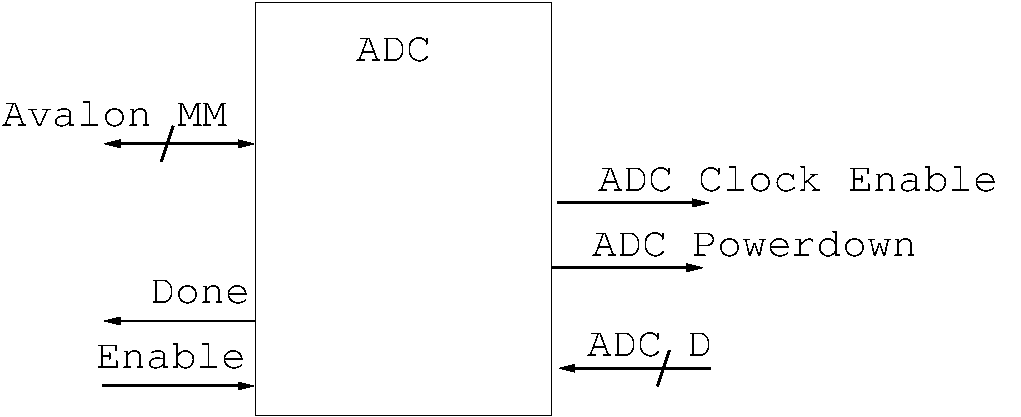
\includegraphics[width=0.4\textwidth]{adc_periph}
\caption{Black box overview of the ADC module}
\label{figure:adc_blackbox}
\end{center}
\end{figure}

The module is enabled by asserting the \texttt{enable} signal for one clock cycle. When
the module completes the sampling, it asserts the \texttt{done} signal until it is enabled
again.

The \texttt{enable} and \texttt{done} signals are connected to the ADC interface
in the SoPC, as described in the SoPC section.


Figure \ref{figure:state_adc} shows a simplified state diagram of the ADC module's state
machine. The module starts up in the \texttt{END} state. While in this state, the
ADC powerdown signal remains asserted, putting the ADC chip into low power mode. In this
state the ADC clock enable signal is deasserted, so that the clock to the ADC is gated.

\begin{figure}[h!]
\begin{center}
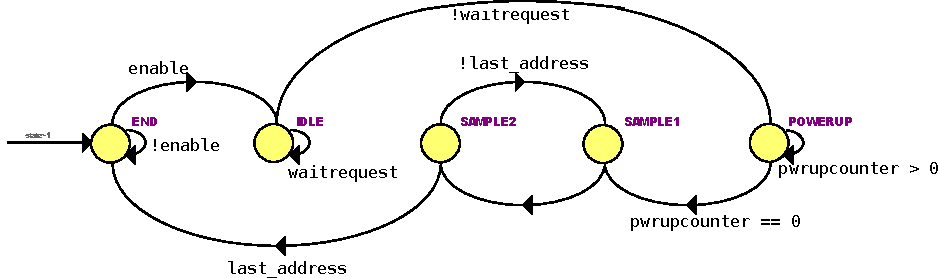
\includegraphics[width=\textwidth]{state_adc}
\caption{Simple state diagram of the ADC module}
\label{figure:state_adc}
\end{center}
\end{figure}

When the external \texttt{enable} signal is asserted, the module transitions into the
\texttt{IDLE} state, where it stays until the SRAM arbiter deasserts the \texttt{mem\_waitrequest}
signal. As soon as the SRAM is ready, the module transitions into the \texttt{POWERUP} state
which ensures that the ADC has enough time after deasserting the powerdown signal to
get back into normal operating mode.

After the ADC has fully powered up, the module transitions between the \texttt{SAMPLE1} and
\texttt{SAMPLE2} states, taking a sample during each and storing it into the upper and lower
bytes of a 16-bit register, respectively.

During the \texttt{SAMPLE2} state, this 16 bit register is written out to SRAM via the
Avalon MM interface to the SRAM arbiter.

As soon as the SRAM is full the module transitions back into the \texttt{END} state, in which
the \texttt{done} signal is asserted notifying the ADC interface in the SoPC that the ADC
module has finished sampling and the ADC is powered down.


\newpage
\section{FPGA Resource usage}
\begin{table}[h!]
\centering
\begin{tabular}{ | p{2cm} | r | r | r | }
 \hline
   Module & Logic cells & DSP Elements & Memory bits \\
 \hline
   SoPC & 17453 & 4 & 1,218,729 \\
 \hline
   ADC & 62 & 0 & 0\\
 \hline
   SRAM Arbiter & 143 & 0 & 298,416 \\
 \hline
   stim & 213 & 0 & 0 \\
 \hline
   check & 122 & 0 & 0 \\
 \hline
   FIFOs & 235 & 0 & 2,544 \\
 \hline
   dut\_if & 149 & 0 & 0 \\
 \hline
 \hline
   Total & 18999 & 4 & 1,221,417 \\
 \hline
\end{tabular}
\caption{FPGA resource usage by module, only including the main modules}
\label{table:resusage}
\end{table}
